\documentclass{beamer}

\mode<presentation> {

% The Beamer class comes with a number of default slide themes
% which change the colors and layouts of slides. Below this is a list
% of all the themes, uncomment each in turn to see what they look like.

%\usetheme{default}
%\usetheme{AnnArbor}
%\usetheme{Antibes}
%\usetheme{Bergen}
%\usetheme{Berkeley}
%\usetheme{Berlin}
%\usetheme{Boadilla}
%\usetheme{CambridgeUS}
%\usetheme{Copenhagen}
%\usetheme{Darmstadt}
%\usetheme{Dresden}
\usetheme{Frankfurt}
%\usetheme{Goettingen}
%\usetheme{Hannover}
%\usetheme{Ilmenau}
%\usetheme{JuanLesPins}
%\usetheme{Luebeck}
%\usetheme{Madrid}
%\usetheme{Malmoe}
%\usetheme{Marburg}
%\usetheme{Montpellier}
%\usetheme{PaloAlto}
%\usetheme{Pittsburgh}
%\usetheme{Rochester}
%\usetheme{Singapore}
%\usetheme{Szeged}
%\usetheme{Warsaw}

% As well as themes, the Beamer class has a number of color themes
% for any slide theme. Uncomment each of these in turn to see how it
% changes the colors of your current slide theme.

%\usecolortheme{albatross}
%\usecolortheme{beaver}
%\usecolortheme{beetle}
\usecolortheme{crane}
%\usecolortheme{dolphin}
%\usecolortheme{dove}
%\usecolortheme{fly}
%\usecolortheme{lily}
%\usecolortheme{orchid}
%\usecolortheme{rose}
%\usecolortheme{seagull}
%\usecolortheme{seahorse}
%\usecolortheme{whale}
%\usecolortheme{wolverine}

%\setbeamertemplate{footline} % To remove the footer line in all slides uncomment this line
%\setbeamertemplate{footline}[page number] % To replace the footer line in all slides with a simple slide count uncomment this line

%\setbeamertemplate{navigation symbols}{} % To remove the navigation symbols from the bottom of all slides uncomment this line
}

\usepackage{extpfeil}
\usepackage{extarrows} %Allows long equation signs
\usepackage{graphicx} % Allows including images
\usepackage{booktabs} % Allows the use of \toprule, \midrule and \bottomrule in tables
\usepackage{physics}
\usepackage{tikz}
\usepackage{cite}
%花体字母
\usepackage{amsthm,amsmath,amssymb}
\usepackage{mathrsfs}
\usepackage{dutchcal}
\usepackage{circuitikz}

%----------------------------------------------------------------------------------------
%	TITLE PAGE
%----------------------------------------------------------------------------------------

\title[VP260 RC]{VP260 Recitation Class 4} % The short title appears at the bottom of every slide, the full title is only on the title page

\author{Yanjun Chen} % Your name
\institute[UM-SJTU JI] % Your institution as it will appear on the bottom of every slide, may be shorthand to save space
{
    University of Michigan - Shanghai Jiao Tong University Joint Institute\\% Your institution for the title page
\medskip
}
\date{\today} % Date, can be changed to a custom date

\begin{document}

\begin{frame}
    \titlepage % Print the title page as the first slide
\end{frame}

%----------------------------------------------------------------------------------------
%	 SECTION 1
%----------------------------------------------------------------------------------------

\section{Fundamental Concepts} % Section title slide, unnumbered

%------------------------------------------------

\begin{frame}{Kirchhoff's Rule}
    \begin{block}{Kirchhoff's rule}
        \begin{itemize}
            \item Junction rule (KCL):
                \begin{equation}
                    \sum_k I_k = 0
                \end{equation}
                where $I_k$ represents a current flows into the junction.
            \item Loop rule (KVL):
                \begin{equation}
                    \sum_k V_k = 0
                \end{equation}
                where $V_k$ represents the voltage across the element in a loop
        \end{itemize}.
    \end{block}
\end{frame}

\begin{frame}{Ammeter and voltmeter}
    An ideal ammeter has zero resistance and an ideal voltmeter has infinitely large resistance.
    
    But in real world, two measurements for R don't give you the same result.

    \vfill

    \begin{columns}
        \begin{column}{.4\linewidth}
            \begin{circuitikz}[american]
                \draw (0,0) -- ++(1,0) to[R] ++(2,0)
                to [rmeter, t=A] ++(2, 0);
                \draw (1,0) -- (1,1) to[rmeter, t=V] ++(2,0) -- (3,0);
            \end{circuitikz}
        \end{column}

        \begin{column}{.4\linewidth}
            \begin{circuitikz}[american]
                \draw (0,0) -- ++(1,0) to[R] ++(2,0)
                to [rmeter, t=A] ++(1, 0) -- ++(1,0);
                \draw (1,0) -- (1,1) to[rmeter, t=V] ++(3.5,0) -- (4.5,0);
            \end{circuitikz}
        \end{column}
    \end{columns}

\end{frame}


\begin{frame}{Direct Current RC Circuits}
    \begin{columns}
        \begin{column}{.5\linewidth}
            \begin{block}{Charging}
                \begin{center}
                    \begin{circuitikz}
                        \draw (0,0) to[battery1=$\epsilon$] (4,0) -- (4,2) to[R=$R$](2,2) -- (1.5,2) to[C=$C$] (0,2) -- (0,0);
                    \end{circuitikz}
                \end{center}
            \end{block}
        \end{column}

        \begin{column}{.5\linewidth}
            \begin{block}{Discharging}
                \begin{center}
                    \begin{circuitikz}
                        \draw (0,0) to[R=$R$] (4,0) -- (4,2) to[C=$C$] (0,2) -- (0,0);
                    \end{circuitikz}
                \end{center}
            \end{block}
        \end{column}
    \end{columns}
\end{frame}


\begin{frame}{Wheatstone bridge circuit}
    We can use this circuit to measure the resistance of $R_x$.

    \begin{center}
        \begin{circuitikz}
            \draw (0,0) -- ++(0,3) to[vR=$R_x$] ++(2,2) -- ++(0,0) to[R=$R_4$] ++(2,-2) -- ++(0,0)to[R=$R_3$] ++(-2,-2) -- ++(0,0)to[R=$R_2$] ++(-2,2);
            \draw (2,5) to[rmeter, t=G] ++(0,-4);
            \draw (4,3) -- ++(0,-3);
            \draw (0,0) to[battery] (4,0);
        \end{circuitikz}
    \end{center}
\end{frame}


\begin{frame}{Magnetic field}
    The basic phenomena of magnetic field:
    \begin{itemize}
        \item Magnets always have two poles;
        \item A wire carrying current will have an impact on a nearby magnet;
        \item Two current-carrying wires will have an impact on each other.
    \end{itemize}
\end{frame}

\begin{frame}{Magnetic Force}
    \begin{block}{Lorentz force}
        \begin{equation}
            \va{F} = q (\va{v} \crossproduct \va{B})
        \end{equation}
    \end{block}
    \begin{itemize}
        \item Magnetic forces do no work.
    \end{itemize}
    \vfill
    \begin{block}{Ampere's force}
        The magnetic force on a segment of current-carrying wire is,
        \begin{equation}
            \va{F} = \int (\va{v} \crossproduct \va{B}) \dd{q} = \int I (\dd{\va{l} \crossproduct \va{B}})
        \end{equation}
    \end{block}
    \begin{itemize}
        \item It seems that Ampere's force does work. Why?
    \end{itemize}
\end{frame}

\begin{frame}{Magnetic Dipole Moment}
    Define the magnetic dipole moment for this current loop:
    \begin{columns}
        \begin{column}{.4\linewidth}
            \begin{figure}[htbp]
                \centering
                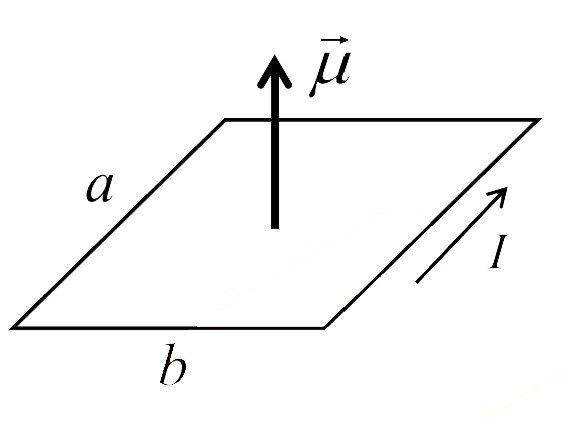
\includegraphics[width=\textwidth]{Images/dipole.jpg}
            \end{figure}
        \end{column}
        \begin{column}{.6\linewidth}
            magnitude: $$\abs{\va{\mu}} = I \times \text{ area} = Iab$$
            direction: right hand rule
        \end{column}
    \end{columns}
    \vfill
    \begin{itemize}
        \item Net torque: $\va{\tau} = \va{\mu} \crossproduct \va{B}$;
        \item Potential energy: $U = -\va{\mu} \vdot \va{B}$
    \end{itemize}
\end{frame}

\begin{frame}{Magnetic Fluxa and Gauss' Law}
    \begin{block}{Magnetic flux}
        \begin{equation}
            \Phi_B = \int_\Sigma \va{B} \vdot \dd{\va{A}}
        \end{equation}
    \end{block}
    \begin{itemize}
        \item Unit: Weber [Wb]
    \end{itemize}
    \vfill
    \begin{block}{Gauss' law for the magnetic field}
        For any closed surface $\Sigma$,
        \begin{equation}
            \Phi_B = \oint_\Sigma \va{B} \vdot \dd{\va{A}} = 0
        \end{equation}
        Hence,
        \begin{equation}
            \div{\va{B}} = 0
        \end{equation}
    \end{block}
    \begin{itemize}
        \item No magnetic monopole (magnetic charge) exists.
    \end{itemize}
\end{frame}



%----------------------------------------------------------------------------------------
%	 Section 2
%----------------------------------------------------------------------------------------

\section{Exercise}

\begin{frame}{Exercise 1}
    In the circuit shown below the batteries have negligible internal resistance and the meters are both idealized. With the switch S open, the voltmeter reads 15.0 V. 
    (a) Find the emf of the battery.
    (b) What will the ammeter read when the switch is closed?

    \begin{figure}[htbp]
        \centering
        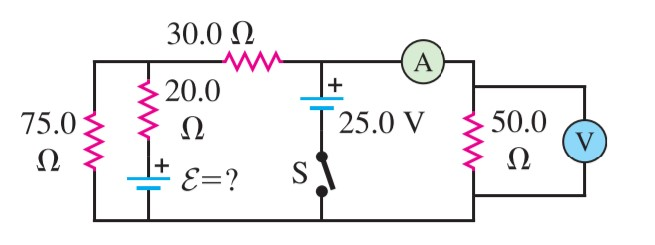
\includegraphics[]{Images/ex1.jpg}    
    \end{figure}
\end{frame}

\begin{frame}{Exercise 2}
    Calculate the resistance between point a and b.
    \begin{figure}[htbp]
        \centering
        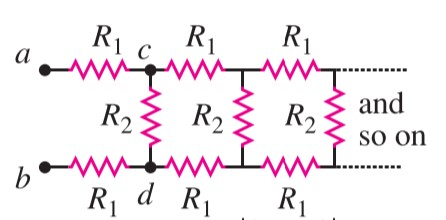
\includegraphics[]{Images/ex2.jpg}    
    \end{figure}

\end{frame}

\begin{frame}{Exercise 3}
    A rectangular loop of wire, supporting a mass $m$, hangs vertically with one end in a uniform magnetic field $\va{B}$, which points into the page in the shaded region. For what current $I$, in the loop, would the magnetic force upward exactly balance the gravitational force downward?.

    \begin{figure}[htbp]
        \centering
        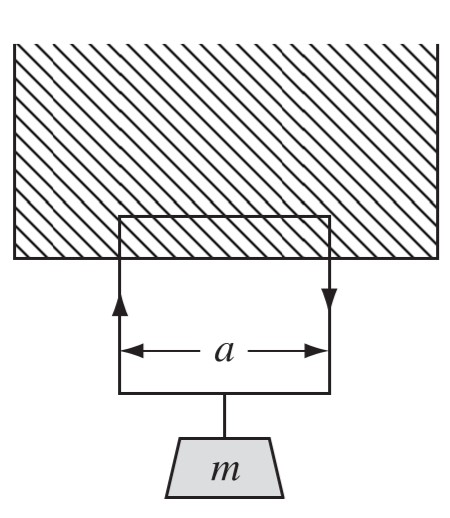
\includegraphics[width=.3\textwidth]{Images/ex3.jpg}
    \end{figure}
\end{frame}

\begin{frame}{Exercise 4}
    A particle of charge $q$ enters a region of uniform magnetic field $\va{B}$ (pointing into the page). The field deflects the particle a distance $d$ above the original line of flight.Is the charge positive or negative? In terms of $a$, $d$, $\va{B}$ and $q$, find the momentum of the particle.

    \begin{figure}[htbp]
        \centering
        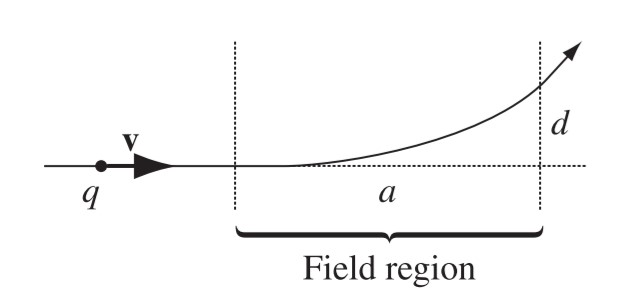
\includegraphics[]{Images/ex4.jpg}    
    \end{figure}
\end{frame}

%----------------------------------------------------------------------------------------
%	 CLOSING/SUPPLEMENTARY SLIDES
%----------------------------------------------------------------------------------------

\begin{frame}
    \begin{center}
        \LARGE\bf Thanks for listening!
    \end{center}
	
\end{frame}


\section{Appendix}

%----------------------------------------------------------------------------------------

\begin{frame}{\bf References}
	\nocite{*} % Display all references regardless of if they were cited
	\bibliography{example.bib}
	\bibliographystyle{plain}
\end{frame}

\end{document}

